% ===================
% Paquetes utilizados
% ===================

% ---------------------
% Clases de documentos: article, report or book.
% Tamaño de fuente: 10pt (default), 11pt o 12pt.
% Tamaño de papel: a4 paper(default), letterpaper, a5paper, b5paper, executivepaper, legalpaper.
% Número de columnas: una columna (predeterminado) o dos columnas.
% ---------------------

\documentclass[11pt,a4paper]{article}
%\usepackage{multicol}

% ---------------------
% "inputenc" es un paquete para traducir varios estándares y otras codificaciones de entrada a un 'lenguaje interno de LaTeX'. 
% El lenguaje interno se expresa completamente en la codificación base de TeX
% (caracteres imprimibles ASCII estándar, tokens de control de carro y secuencias de control de TeX, estas últimas definidas principalmente por LaTeX).
% ---------------------

\usepackage[utf8]{inputenc}

% ---------------------
% Para cambiar la fuente. 
% Para el caso estándar, elimine las dos últimas líneas.
% ---------------------

\usepackage[T1]{fontenc}
\usepackage{libertine}
\usepackage{libertinust1math}

% ---------------------
% Paquete para redefinir el comando \author para que funcione normalmente o para permitir un estilo de nota al pie de entrada de autor/afiliación.
% ---------------------

\usepackage{authblk}

% ---------------------
% Este paquete busca pdfTeX en modo pdf e implementa y configura el modificador \ifpdf. 
% La detección se basa en el valor de \pdfoutput (que el paquete no cambiará). El paquete funciona con formatos planos o LaTeX. 
% Para usarlo con LaTeX simplemente \usepackage{ifpdf}. Luego use \ifpdf ... \else ... \fi.
% ---------------------

\usepackage{ifpdf}
\newif\ifpdf\ifx\pdfoutput\undefined\pdffalse\else\pdfoutput=1\pdftrue\fi

% ---------------------
% Para que alternativamente se puedan usar figuras en pdf o jpg.
% ---------------------

\newcommand{\pdfgraphics}{\ifpdf\DeclareGraphicsExtensions{.pdf,.jpg}\fi}

% ---------------------
% Para proporcionar los medios para componer texto en español, con el soporte provisto por el paquete estándar de LaTeX babel.
% ---------------------

\usepackage[spanish,es-tabla]{babel}

% ---------------------
% "hyperref" se usa para manejar comandos de referencias cruzadas en LaTeX para producir enlaces de hipertexto en el documento.
\usepackage{hyperref}
\hypersetup{colorlinks=true, linkcolor=black, filecolor=black, urlcolor=blue, citecolor=blue}
% ---------------------

% ---------------------
% Funciones matematicas.
% Notación de bra-ket de Dirac.
% Notación tensorial (índices).
% Diagramas de Feynman.
% Para escribir algoritmos en pseudocódigo.
% Para escribir algoritmos en distintos lenguajes de programacion.
% ---------------------

\usepackage{amsmath}
\usepackage{braket}
\usepackage{slashed}
\usepackage{tensor}
\usepackage{tikz-feynman}
\usepackage[spanish,onelanguage,ruled,vlined,boxed]{algorithm2e}

\usepackage{listings}
\usepackage{xcolor}

\definecolor{codegreen}{rgb}{0,0.6,0}
\definecolor{codegray}{rgb}{0.5,0.5,0.5}
\definecolor{codepurple}{rgb}{0.58,0,0.82}
\definecolor{backcolour}{rgb}{0.95,0.95,0.92}

\lstdefinestyle{mystyle}{
    backgroundcolor=\color{backcolour},   
    commentstyle=\color{codegreen},
    keywordstyle=\color{magenta},
    numberstyle=\tiny\color{codegray},
    stringstyle=\color{codepurple},
    basicstyle=\ttfamily\footnotesize,
    breakatwhitespace=false,         
    breaklines=true,                 
    captionpos=b,                    
    keepspaces=true,                 
    numbers=left,                    
    numbersep=5pt,                  
    showspaces=false,                
    showstringspaces=false,
    showtabs=false,                  
    tabsize=2
}

\lstset{style=mystyle}

% ---------------------
% Fuentes para usar en matemáticas.
% ---------------------

\usepackage{amsfonts}

% ---------------------
% Para insertar imágenes.
% Posicionamiento flotante de figuras y tablas.
% Para comentar (captions) las figuras.
% ---------------------

\usepackage{graphicx}
\usepackage{afterpage}
\usepackage{float}
\usepackage{subcaption}

% ---------------------
% Bibliografía con bibtex.
% Encabezados y pies de página.
% Para dar formato a los títulos de los apéndices.
% ---------------------

\bibliographystyle{unsrt}
\usepackage{fancyhdr}
\usepackage[hang,flushmargin]{footmisc} % Para configurar notas al pie de página
\usepackage{appendix}

% ---------------------
% Configuración de longitudes.
% ---------------------

\setlength{\oddsidemargin}{0in}
\setlength{\textwidth}{6in}
\setlength{\topmargin}{0in}
\setlength{\voffset}{-0.5in}
\setlength{\hoffset}{0.5in}
\setlength{\textheight}{9in}
\setlength{\textwidth}{6in}
\setlength{\topskip}{0in}
\setlength{\parskip}{2ex}

\renewcommand{\arraystretch}{1.0}
\renewcommand{\baselinestretch}{1.0}

% ---------------------
% Para definir un nuevo encabezado para todas las páginas.
% ---------------------

\fancypagestyle{plain}{\fancyhf{}\renewcommand{\headrulewidth}{0pt}}

% ---------------------
% Titulo del documento
% ---------------------

\title{\textbf{``Integrales de camino como enfoque alternativo para la valuaci\'on de opciones financieras''} \\ \large \textit{Programa en finanzas cuantitativas - Universidad del CEMA \\ Trabajo Final}}


% ---------------------
% Autor - Institución - Fecha
% ---------------------

\author[1]{\textbf{Rodrigo J. Kang}}
\affil[1]{\normalsize \textit{Facultad de Ciencias Exactas Universidad Nacional de La Plata, C.C 67, 1900 La Plata, Argentina.}}
\date{}

% ---------------------
% Comienzo del documento
% ---------------------

\begin{document}

% ---------------------
% Exteriorizar Titulo - Autor - Institución - Date
% ---------------------

\maketitle

% ---------------------
% Exteriorizar numero de columnas
% ---------------------

%\begin{multicols}{2}

% ---------------------
% Resumen
% ---------------------

\begin{abstract}
En este trabajo proponemos el uso de integrales de camino como una estrategia innovadora y alternativa a los modelos convencionales para fijar precios de opciones financieras. Analizamos el caso de opciones tipo call europeas y obtenemos el propagador de Black-Scholes de manera ana\'itica mediante la aplicaci\'on de integrales funcionales. Haciendo uso de la convoluci\'on del propagador de Black-Scholes contra la funci\'on de payoff ofrecemos una demostraci\'on diferente al teorema fundamental de la valuaci\'on de activos. Por \'ultimo, implementamos el algoritmo de Metropolis-Hasting como m\'etodo num\'erico parra efectuar las integrales multidimensionales que naturalmente aparecen en la formulaci\'on de integral funcional y comparamos los resultados ana\'iticos y num\'ericos.
\end{abstract}

{\setlength{\parindent}{0pt}{\bf Palabras clave:} Integrales de camino, opciones, Black-Scholes, Metropolis-Hasting.}

% ---------------------
% Sección 1
% ---------------------

\section{Introducción}

En 1973 Black y Scholes establecieron las bases de la teor\'ia cl\'asica de fijaci\'on de precios de opciones \cite{black1973pricing}. Ese mismo a\~no e independientemente de Black y Scholes, Merton deriv\'o la misma formulaci\'on \cite{merton1973theory}. Esta teor\'ia se basa en la din\'amica de un proceso estoc\'astico espec\'ifico, el movimiento browniano geom\'etrico. En condiciones ideales de mercado, sin arbitraje, sin dividendos y con volatilidades constantes, la f\'ormula de Black-Scholes-Merton proporciona una soluci\'onn anal\'itica para la valuaci\'on de opciones financieras, especialmente para opciones europeas tipo call simples. Sin embargo, para el caso de derivados financieros m\'as complejos, que se caracterizan por el ejercicio anticipado y la dependencia del historial del activo subyacente, la f\'orrmula Black-Scholes-Merton no ofrece soluciones anal\'iticas, lo cual se ha constitu\'ido en un desaf\'io que ha sido abordado mediante el desarrollo de m\'etodos num\'ericos espec\'ificos para la valuaci\'on de derivados financieros ex\'oticos con caracter\'isticas dependientes de la trayectoria \cite{linetsky1997path, devreese2010path}.\\
En este contexto, este trabajo se enfoca en contribuir a la eficiente valuaci\'on de opciones en el \'ambito financiero mediante el uso del m\'etodo de integral de camino. Este m\'etodo que tiene sus ra\'ices en los trabajos de Wiener y Kac en cálculo estocástico y de Feynman en mecánica cuántica, ha ganado importancia en finanzas \cite{linetsky1997path, devreese2010path, montagna2002path, capuozzo2021path}. Este enfoque permite la aplicaci\'on de t\'ecnicas anal\'iticas y num\'ericas muy potentes y robustas. Debido a la importancia capital de las opciones en los mercados financieros, con un valor de mercado bruto de derivados extraburs\'atiles que super\'o los 15.5 billones de d\'olares en el primer semestre de 2020 \cite{capuozzo2021path}, el desarrollo de modelos y m\'etodos computacionales para la fijaci\'on de precios de opciones es crucial. A pesar de las conocidas deficiencias en los supuestos del modelo Black-Scholes-Merton, su amplio uso persiste, en gran medida debido a la disponibilidad de soluciones cerradas \cite{maurette2023quantderivados}. Sin embargo, las opciones m\'as exóticas requieren enfoques num\'ericos como diferencias finitas, elementos finitos o Monte Carlo. En este sentido, las integrales de trayectoria ofrecen una formulaci\'on alternativa elegante. Introducidas en los modelos financieros por Dash \cite{dash1989path} y Linetsky \cite{linetsky1997path}, estas integrales, basadas en el trabajo previo de Feynman en mecánica cuántica \cite{feynman2010quantum, sakurai1995modern, falomir2021integrales, schaposnik2014cuantica} y de Wiener en movimiento browniano \cite{wiener1921average}, se han vuelto estándar en matemáticas financieras.\\
Este trabajo se organiza de la siguiente manera. En la Secci\'on 2 se introduce el concepto de integral de camino en el contexto de la mec\'anica cu\'antica como herramienta para calcular la amplitud de probabilidad entre un estado inicial y un estado final y su relaci\'on con la funci\'on de Green de la ecuación de Schr\"odinger. En la Secci\'on 3 se analiza la relaci\'on que existe entre la din\'amica del mercado de opciones y la de los sistemas cu\'anticos, se deriva el propagador de Black-Scholes de manera anal\'itica aplicando el enfoque de integrales de trayectoria y se muestra c\'omo con esta formulaci\'on es posible obtener el teorema fundamental de la valuación de activos. En la Secci\'on 3 se argumenta el motivo por el cual el algoritmo de Metropolis-Hasting es el m\'etodo num\'erico m\'as adecuado para realizar las integrales multidimensionales que emergen de la formulaci\'on de la integral funcional y se presentan los resultados obtenidos de la implementaci\'on de este algoritmo con el lenguaje de programaci\'on Python. Por \'ultimo, se cierra este trabajo con conclusiones y posibles perspectivas.

\section{Integrales de camino en mec\'anica cu\'antica}

En mec\'anica cu\'antica, los estados de un sistema est\'an descritos por funciones de onda que son vectores en un espacio de Hilbert $\mathcal{H}$ y cuya din\'amica (en el caso no relativista) est\'a dada por la ecuaci\'on de Schrödinger. Sin p\'erdida de generalidad y con el objetivo de simplificar los c\'alculos, consideremos un sistema cu\'antico con un \'unico grado de libertad. En este contexto, para un hamiltoniano dado $\hat{H}$, la ecuaci\'on de Schrödinger toma la forma:
\begin{equation}
i \hbar \frac{\partial \psi}{\partial t} = \hat{H} \psi
\label{eq:Schrödinger}
\end{equation}
Si se conoce la función de onda $\psi(x_i,t_i)$ en un momento dado $t_i$, podemos deducir su forma en un momento posterior $t_f$ que es equivalente a integrar la ecuaci\'on (\ref{eq:Schrödinger}). Para ello, es necesario conocer el efecto de la funci\'on de onda $\psi(x_i,t_i)$ en el instante incial $t_i$ sobre la funci\'on de onda $\psi(x_f,t_f)$ en el instante final $t_f$. Es razonable suponer que la intensidad de la onda que surge de $x_i$ y llega a $x_f$ en el momento $t_f$ es proporcional a la amplitud inicial \cite{greiner2008quantum}. Por lo tanto, si llamamos $K(x_f,t_f;x_i,t_i)$ a la constante de proporcionalidad y consideramos todas las contribuciones en cada punto del espacio desde el instante inicial al instante final, la soluci\'on a la ecuaci\'on de (\ref{eq:Schrödinger}) puede expresarse como:
\begin{equation}
\psi(x_f,t_f)= \int_{-\infty}^{\infty} \mathrm{d}x_i \; K(x_f,t_f; x_i,t_i) \; \psi(x_i,t_i)
\label{eq:Propagator1}
\end{equation}
La cantidad $K(x_f,t_f; x_i,t_i)$ se conoce como función de Green o propagador y dado que describe el efecto de la onda $\psi(x_i,t_i)$, que se encontraba en el punto $x_i$ en el pasado $t_i$, sobre la onda $\psi(x_f,t_f)$, que se encuentra en el punto $x_f$ en el momento posterior $t_f$, el conocimiento de la evoluci\'on temporal del sistema cu\'antico se reduce a determinar la forma de $K(x_f,t_f; x_i,t_i)$.\\
En lo que sigue vamos a calcular el propagador usando el m\'etodo de integrales de camino propuesto por Feynman\footnote{Originalemte la idea fue propuesta por Dirac y sistematizada por Feynman \cite{schaposnik2014cuantica}.}, para ello destacamos el hecho de que la funci\'on de onda en el esquema de Schr\"odinger\footnote{En el esquema de Schr\"odinger los estados de un sistema cu\'antico est\'an descritos por vectores de un espacio de Hilbert $\mathcal{H}$ que evolucionan con el tiempo mientras que los operadores son independientes del tiempo. Por otra parte, en el esquema de Heisenberg, el estado est\'a determinado por un vector fijo de $\mathcal{H}$, mientras que los operadores evolucionan con el tiempo \cite{sakurai1995modern, falomir2021integrales, schaposnik2014cuantica}.} en la representaci\'on de coordenadas se escribe como\footnote{Dada una base de autofunciones del operador posición, el estado cu\'antico $\ket{\psi}$ se puede representar como una combinación lineal de los estados de dicha base:
\begin{equation}
\ket{\psi}= \int \mathrm{d}x_f \;\ket{x_f}\braket{x_f|\psi}
\label{eq:representation1}
\end{equation}
Se dice entonces que el valor de la funci\'on de onda en $x_f$, es la componente del estado $\ket{\psi}$ sobre el vector base $\ket{x_f}$ de la representaci\'on $\{ \ket{x_f} \}$ \cite{cohen1986quantum}, es decir:
\begin{equation}
\psi(x_f) = \braket{x_f|\psi}
\label{eq:representation2}
\end{equation}
An\'alogamente se puede definir el valor de la funci\'on de onda en la representaci\'on de momentos.}:
\begin{equation}
\psi(x_f,t_f) = \braket{x_f|\psi;t_f}
\label{eq:wavefunction}
\end{equation}
dado que los dos estados $\ket{\psi;t_f}$ y $\ket{\psi;t_i}$ est\'an conectados por el operador evoluci\'on $\hat{U}(t_f,t_i)$:
\begin{equation}
\ket{\psi;t_f} = \hat{U}(t_f,t_i)\ket{\psi;t_i}
\label{eq:evolution}
\end{equation}
la ecuaci\'on (\ref{eq:wavefunction}) se puede entender como el elemento de matriz del operador evoluci\'on temporal, es decir:
\begin{equation}
\psi(x_f,t_f) = \braket{x_f|\psi;t_f} = \bra{x_f}\hat{U}(t_f,t_i)\ket{\psi_i;t_i} = \int \mathrm{d}x_i \bra{x_f}\hat{U}(t_f,t_i)\ket{x_i}\psi(x_i,t_i) 
\label{eq:matrixelement}
\end{equation}
con lo que comparando la ecuaci\'on (\ref{eq:matrixelement}) con la ecuaci\'on (\ref{eq:Propagator1}) podemos identificar el propagador como $K(x_f,t_f; x_i,t_i) := \bra{x_f}\hat{U}(t_f,t_i)\ket{x_i}$, que no es otra cosa que la amplitud de probabilidad de transici\'on entre un estado inicial $(x_i,t_i)$ y un estado final $(x_f,t_f)$. \\
Para un Hamiltoniano que no tenga una depencia expl\'icita del tiempo, se puede ver que el operador evoluci\'on est\'a dado por \cite{falomir2021integrales}:
\begin{equation}
\hat{U}(t_f,t_i) = e^{-\frac{i}{\hbar}\hat{H} (t_f - t_i)}
\label{eq:evolutionoperator}
\end{equation}
luego,
\begin{equation}
K(x_f,t_f; x_i,t_i) := \bra{x_f}\hat{U}(t_f,t_i)\ket{x_i} = \bra{x_f}e^{-\frac{i}{\hbar}\hat{H} (t_f - t_i)}\ket{x_i}
\label{eq:Propagator2}
\end{equation}
Para poder llevar a cabo este c\'alculo lo que podemos hacer es fraccionar el intervalo temporal en $N \in \mathbb{N}$ intervalos discretos de longitud $\Delta t = \frac{t_f - t_i}{N}$, con lo cual:
\begin{equation}
\bra{x_f}e^{-\frac{i}{\hbar}\hat{H} (t_f - t_i)}\ket{x_i} = \bra{x_f}\prod_{k=1}^N e^{-\frac{i}{\hbar}\hat{H}\Delta t}\ket{x_i}
\label{eq:Propagator3}
\end{equation}
Teniendo en cuenta que los operadores $\hat{p}$ y $\hat{x}$ tienen sistemas completos de autovectores:
\begin{equation}
\begin{split}
& \hat{p}\ket{p} = p\ket{p}, \; p \in \mathbb{R}, \; \; \hat{I} = \int \mathrm{d}p \ket{p}\bra{p} \\
& \hat{x}\ket{x} = x\ket{x}, \; x \in \mathbb{R}, \; \; \hat{I} = \int \mathrm{d}x \ket{x}\bra{x}
\end{split}
\label{eq:eigenvectors}
\end{equation}
podemos usar estas relaciones de clausura para reescribir la ecuaci\'on (\ref{eq:Propagator3}) de la siguiente forma:
\begin{equation}
\begin{split}
\bra{x_f}e^{-\frac{i}{\hbar}\hat{H} (t_f - t_i)}\ket{x_i} = \int \mathrm{d}x_1 \int \mathrm{d}x_2 \cdots \int \mathrm{d}x_{N-1} & \bra{x_N}e^{-\frac{i}{\hbar}\hat{H}\Delta t}\ket{x_{N-1}} \bra{x_{N-1}}e^{-\frac{i}{\hbar}\hat{H}\Delta t}\ket{x_{N-2}} \\
& \cdots \bra{x_2}e^{-\frac{i}{\hbar}\hat{H}\Delta t}\ket{x_1} \bra{x_1}e^{-\frac{i}{\hbar}\hat{H}\Delta t}\ket{x_0}
\end{split}
\label{eq:Propagator4}
\end{equation}
identificando $x_0 = x_i$ y $x_N = x_f$. Adem\'as, el operador hamiltoniano est\'a dado por:
\begin{equation}
\hat{H}(\hat{p},\hat{x}) = \frac{\hat{p}^2}{2m} + V(\hat{x})
\label{eq:hamiltonian}
\end{equation}
Con lo que bas\'andonos en la aproximaci\'on a orden $(\Delta t)^2$ (i.e. $\mathcal{O}(N^{-2})$) de la f\'ormula de Baker-Campbell-Hausdorff\footnote{
\begin{equation}
e^{\hat{X} + \hat{Y}} = e^{\hat{X}}e^{\hat{Y}}e^{-\frac{1}{2}[\hat{X},\hat{Y}] + \cdots}
\label{eq:haussdorf}
\end{equation}}
podemos escribir:
\begin{equation}
e^{-\frac{i}{\hbar}\hat{H}\Delta t} = e^{-\frac{i}{\hbar}\frac{\hat{p}^2}{2m}\Delta t} e^{-\frac{i}{\hbar}V(\hat{x})\Delta t} e^{-\frac{1}{2}\left( \frac{-i\Delta t}{\hbar} \right)^2\left[\frac{\hat{p}^2}{2m}, V(\hat{x})\right] + \cdots}
\label{eq:Propagator5}
\end{equation}
A partir de esto, suponiendo suavidad en la funci\'on $V(\hat{x})$ respecto a su argumento y teniendo en cuenta que:
\begin{equation}
\braket{x|p} = \frac{e^{\frac{i}{\hbar}px}}{\sqrt{2\pi\hbar}}
\label{eq:braxketp}
\end{equation}
obtenemos la siguiente aproximaci\'on:
\begin{equation}
\begin{split}
\bra{x_{j+1}}e^{-\frac{i}{\hbar}\hat{H}\Delta t}\ket{x_j} & = \bra{x_{j+1}}e^{-\frac{i}{\hbar}\frac{\hat{p}^2}{2m}\Delta t} e^{-\frac{i}{\hbar}V(\hat{x})\Delta t} \ket{x_j} \left[ 1 + \mathcal{O}\left( N^{-2} \right) \right] \\
& = \int_{-\infty}^{\infty}dp_j \braket{x_{j+1}|p_j}e^{-\frac{i}{\hbar}\frac{p_{j}^2}{2m}\Delta t}\braket{p_j|x_j}e^{-\frac{i}{\hbar}V(x_j)\Delta t}\left[ 1 + \mathcal{O}\left( N^{-2} \right) \right] \\
& = \int_{-\infty}^{\infty}\frac{dp_j}{2\pi\hbar} e^{\frac{i}{\hbar}p(x_{j+1}-x_j)} e^{-\frac{i}{\hbar}\frac{p_{j}^2}{2m}\Delta t}e^{-\frac{i}{\hbar}V(x_j)\Delta t}\left[ 1 + \mathcal{O}\left( N^{-2} \right) \right] \\
& = \int_{-\infty}^{\infty}\frac{dp_j}{2\pi\hbar} e^{\frac{i}{\hbar}\left[p_j\left( \frac{x_{j+1}-x_j}{\Delta t} \right) - H(p_j,x_j)\right]\Delta t } \left[ 1 + \mathcal{O} \left( N^{-2} \right) \right]
\label{eq:Propagator6}
\end{split}
\end{equation}
donde la funci\'on $H(p,x)$ es el hamiltoniano cl\'asico del sistema, es decir:
\begin{equation}
H(p,x) = \frac{p^2}{2m} + V(x)
\label{eq:classicamiltonian}
\end{equation}
insertando el resultado (\ref{eq:Propagator6}) en la ecuaci\'on (\ref{eq:Propagator4}) tenemos que:
\begin{equation}
\begin{split}
\bra{x_f}e^{-\frac{i}{\hbar}\hat{H} (t_f - t_i)}\ket{x_i} = & \int \mathrm{d}x_1 \int \mathrm{d}x_2 \cdots \int \mathrm{d}x_{N-1} \int \frac{\mathrm{d}p_0}{2\pi\hbar} \int \frac{\mathrm{d}p_1}{2\pi\hbar} \cdots \int \frac{\mathrm{d}p_{N-1}}{2\pi\hbar} \\
& e^{\frac{i}{\hbar}\sum_{j=0}^{N-1}\Delta t\left[p_j\left( \frac{x_{j+1}-x_j}{\Delta t} \right) - H(p_j,x_j)\right]} \left[ 1 + \mathcal{O} \left( N^{-2} \right) \right]^N \\
= & \int \mathrm{d}x_1 \int \mathrm{d}x_2 \cdots \int \mathrm{d}x_{N-1} \int \frac{\mathrm{d}p_0}{2\pi\hbar} \int \frac{\mathrm{d}p_1}{2\pi\hbar} \cdots \int \frac{\mathrm{d}p_{N-1}}{2\pi\hbar} \\
& e^{\frac{i}{\hbar}\sum_{j=0}^{N-1}\Delta t\left[p_j\left( \frac{x_{j+1}-x_j}{\Delta t} \right) - H(p_j,x_j)\right]} \left[ 1 + \mathcal{O} \left( N^{-1} \right) \right]
\end{split}
\label{eq:Propagator7}
\end{equation}
tomando el l\'imite con $N$ tendiendo a infinito obtenemos una forma de calcular la amplitud de probabilidad y por lo tanto el propagador:
\begin{equation}
\begin{split}
K(x_f,t_f; x_i,t_i) & = \bra{x_f}e^{-\frac{i}{\hbar}\hat{H} (t_f - t_i)}\ket{x_i} \\
& = \lim_{N\rightarrow \infty}\int \mathrm{d}x_1 \cdots \int \mathrm{d}x_{N-1} \int \frac{\mathrm{d}p_0}{2\pi\hbar} \cdots \int \frac{\mathrm{d}p_{N-1}}{2\pi\hbar} \\
& e^{\frac{i}{\hbar}\sum_{j=0}^{N-1}\Delta t\left[p_j\left( \frac{x_{j+1}-x_j}{\Delta t} \right) - H(p_j,x_j)\right]} \left[ 1 + \mathcal{O} \left( N^{-1} \right) \right] \\
& = \int\mathcal{D}x\mathcal{D}p \; e^{\frac{i}{\hbar}\int_{t_i}^{t_f}\mathrm{d}t\left[ p(t)\dot{x}(t)-H(p(t),x(t))\right]}
\end{split}
\label{eq:Propagator8}
\end{equation}
donde hemos introducido la siguiente medida de integración:
\begin{equation}
\mathcal{D}x\mathcal{D}p = \lim_{N \rightarrow \infty}\left( \prod_{k=1}^{N-1}\mathrm{d}x_k\frac{\mathrm{d}p_k}{2\pi\hbar} \right)\frac{\mathrm{d}p_0}{2\pi\hbar}
\label{eq:measure}
\end{equation}
Es inmediato identificar el exponente con la acci\'on cl\'asica, es decir:
\begin{equation}
S\left[ p(t), x(t) \right] := \int_{t_i}^{t_f}\mathrm{d}t\left[ p(t)\dot{x}(t) - H(p(t),x(t)) \right] 
\label{eq:action}
\end{equation}
con lo cual:
\begin{equation}
K(x_f,t_f; x_i,t_i) = \int\mathcal{D}x\mathcal{D}p \; e^{\frac{i}{\hbar}S\left[ p(t), x(t) \right]}
\label{eq:Propagator9}
\end{equation}
que puede interpretarse como la suma ponderada por las contribuciones provenientes de la exponencial de $\frac{i}{\hbar}$ veces la acci\'on cl\'asica (en la formulaci\'on Hamiltoniana) de aquellos caminos del espacio de fases $(p(t),x(t))$ que conectan los puntos $x_i$ y $x_f$ en la ventana temporal $(t_f - t_i)$.\\
Por otro lado, dado que las variables $p_j$ en la ecuaci\'on (\ref{eq:Propagator8}) pueden ser integradas, la integral de camino puede ser llevada al espacio de configuraci\'on. Para ello, introducimos las siguientes definiciones para compactar un poco la notaci\'on:
\begin{equation}
\left\{
\begin{array}{l}
\Delta x := x_{j+1} - x_j \\ \\
I(\Delta x) : = \int_{-\infty}^{\infty} \frac{dp_j}{2\pi\hbar} e^{\frac{i}{\hbar}\left[ p_j \Delta x - \Delta t \frac{p_j^2}{2m} - \Delta t V(x_j) \right]}
\end{array} 
\right.
\label{eq:definitions}
\end{equation}
si completamos cuadrados:
\begin{equation}
\begin{split}
- \frac{\Delta t}{2m} p_j^2 + \Delta x p_j - \Delta t V(x_j) & = - \frac{\Delta t}{2m} \left[ p_j^2 - \frac{2m\Delta x}{\Delta t} p_j + \left( \frac{m\Delta x}{\Delta t} \right)^2 - \left( \frac{m\Delta x}{\Delta t} \right)^2 \right] - \Delta t V(x_j) \\
&  = - \frac{\Delta t}{2m} \left( p_j - \frac{m \Delta x}{\Delta t} \right)^2 + \frac{m\Delta x}{2 \Delta t} - \Delta t V(x_j)
\end{split}
\label{eq:completingthesquare}
\end{equation}
y sustituimos en la integral $I(\Delta x)$ de la ecuaci\'on (\ref{eq:definitions}) tenemos que:
\begin{equation}
\begin{split}
I(\Delta x) & = \frac{1}{2\pi\hbar}e^{\frac{im\Delta x^2}{2\hbar\Delta t}- \frac{i\Delta t}{\hbar} V(x_j)}\int_{-\infty}^{\infty} dp_j e^{-\frac{i\Delta t}{2m\hbar}\left( p_j - \frac{m\Delta x}{\Delta t}\right)^2} \\
& = \sqrt{\frac{m}{2\pi\hbar i \Delta t}}e^{\frac{i\Delta t}{\hbar}\left[ \frac{m}{2}\left( \frac{\Delta x}{\Delta t} \right)^2 - V(x_j) \right]}
\end{split}
\label{eq:integral}
\end{equation}
con lo cual, reemplazando estas integrales en la expresi\'on (\ref{eq:Propagator8}) obtenemos:
\begin{equation}
\begin{split}
K(x_f,t_f; x_i,t_i) & = \bra{x_f}e^{-\frac{i}{\hbar}\hat{H} (t_f - t_i)}\ket{x_i} \\
& = \lim_{N\rightarrow \infty}\int \mathrm{d}x_1 \cdots \int \mathrm{d}x_{N-1} \left( \frac{m}{2\pi\hbar i \Delta t} \right)^{\frac{N}{2}} e^{\frac{i\Delta t}{\hbar}\sum_{j=0}^{N-1}\left[ \frac{m}{2}\left( \frac{\Delta x}{\Delta t} \right)^2 - V(x_j) \right]} \left[ 1 + \mathcal{O} \left( N^{-1} \right) \right]  \\
& = \int\mathcal{D}x \; e^{\frac{i}{\hbar}\int_{t_i}^{t_f}\mathrm{d}t \; L}
\end{split}
\label{eq:Propagator10}
\end{equation}
donde la cantidad $L = \frac{m}{2}\dot{x}^2(t) - V\left[x(t)\right]$ es el lagrangiano del sistema. Por lo tanto, podemos identificar al exponente con la acci\'on cl\'asica en la formulaci\'on Lagrangiana, es decir:
\begin{equation}
S\left[ x(t) \right] := \int_{t_i}^{t_f}\mathrm{d}t \; L\left[ x(t), \dot{x}(t) \right]
\label{eq:actionlagrangian}
\end{equation}
por lo que el propagador puede expresarse como:
\begin{equation}
K(x_f,t_f; x_i,t_i) = \int\mathcal{D}x \; e^{\frac{i}{\hbar}S\left[ x(t) \right]}
\label{eq:Propagator11}
\end{equation}
y cuya medida de integraci\'on est\'a dada por:
\begin{equation}
\mathcal{D}x = \lim_{N \rightarrow \infty} \prod_{k=1}^{N-1}\mathrm{d}x_k\left( \frac{m}{2\pi\hbar i \Delta t} \right)^{\frac{N}{2}}
\label{eq:measureconfiguration}
\end{equation}
El resultado (\ref{eq:Propagator11}) nos dice que la amplitud de probabilidad se determina mediante la suma de todas las trayectorias (o caminos) continuos en el espacio de configuraci\'on ponderados por las contribuciones de la forma $e^{\frac{i}{\hbar}S\left[ x(t) \right]}$ tomadas con la medida de integraci\'on dada por (\ref{eq:measureconfiguration}) y sujetos a la condici\'on inicial $x(t_i) = x_i$ y la condición final $x(t_f) = x_f$.\\

\section{Analog\'ias entre los sistemas cu\'anticos y los mercados de opciones}

En esta secci\'on explicaremos la conexi\'on sorprendente y profunda que existe entre el comportamiento de los sistemas cu\'anticos y el de los mercados de opciones y c\'omo utilizando el enfoque de integrales funcionales desarrollados en el apartado anterior en el marco de la mec\'anica cu\'antica es posible valuar este tipo de derivados financieros. \\
En primer lugar, consideremos la ecuaci\'on de Black-Scholes para el caso de una call europea en donde $S$ es el precio del activo subyacente y en el que $K$ y $T$ corresponden  al strike price y al tiempo de expiraci\'on respectivamente. Si llamamos $C(S,t)$ al valor de la call europea, la ecuaci\'on de Black-Scholes puede expresarse como: \cite{black1973pricing, merton1973theory, maurette2023quantderivados, ziemann2021quantum}:
\begin{equation}
\frac{\partial C}{\partial t} +\frac{1}{2} \sigma ^2 S^2 \frac{\partial^2 C}{\partial S^2} + rS\frac{\partial C}{\partial S} - rC = 0
\label{eq:blackscholes1}
\end{equation}
Haciendo el cambio de variables $x = \ln(S)$, tenemos las siguientes relaciones:
\begin{equation}
\left\{
\begin{array}{l}
\frac{\partial C}{\partial S} = \frac{\partial C}{\partial x}\frac{dx}{dS} = \frac{1}{S}\frac{\partial C}{\partial x} \\ \\
\frac{\partial^2 C}{\partial S^2} = \frac{\partial}{\partial S}\left( \frac{1}{S} \frac{\partial C}{\partial x} \right) = - \frac{1}{S^2}\frac{\partial C}{\partial x} + \frac{1}{S^2}\frac{\partial^2 C}{\partial x^2}
\end{array}
\right.
\label{eq:changeofvariable}
\end{equation}
con lo que sustituy\'endolas la ecuaci\'on (\ref{eq:blackscholes1}) podemos reescribirla de la siguiente manera:
\begin{equation}
\begin{split}
& \frac{\partial C}{\partial t} + \frac{1}{2} \sigma^2 S^2 \left( - \frac{1}{S^2}\frac{\partial C}{\partial x} + \frac{1}{S^2}\frac{\partial^2 C}{\partial x^2} \right) + rS\left( \frac{1}{S}\frac{\partial C}{\partial x} \right) - rC = 0 \\
& \Rightarrow \frac{\partial C}{\partial t} + \frac{1}{2} \sigma^2 \frac{\partial^2 C}{\partial x^2} - \left( \frac{1}{2} \sigma^2 - r \right)\frac{\partial C}{\partial x} - rC = 0
\end{split}
\label{eq:blackscholes2}
\end{equation}
Separando la parte temporal de la espacial, podemos llevar la ecuaci\'on (\ref{eq:blackscholes2}) a la siguiente forma:
\begin{equation}
\frac{\partial C}{\partial t} = \hat{H}_{BS}C
\label{eq:blackscholes3}
\end{equation}
donde:
\begin{equation}
\hat{H}_{BS} := - \frac{1}{2} \sigma^2 \frac{\partial^2 }{\partial x^2} + \left( \frac{1}{2} \sigma^2 - r \right)\frac{\partial }{\partial x} + r
\label{eq:blackscholes4}
\end{equation}
es el Hamiltoniano de Black-Scholes \cite{ziemann2021quantum}. \\
Es aqu\'i es donde podemos ver la relaci\'on que existe entre la din\'amica de las opciones y la de los sistemas cu\'anticos, dado que comparando la ecuaci\'on (\ref{eq:blackscholes3}) con la ecuaci\'on (\ref{eq:Schrödinger}) nos permite interpretar a la ecuaci\'on de Black-Scholes como la ecuaci\'on de Schr\"odinger dependiente del tiempo transformada seg\'un la prescripci\'on $t \rightarrow \frac{-it}{\hbar}$, que en el contexto de la f\'isica se conoce con el nombre de rotaci\'on de Wick \cite{capuozzo2021path}. Esto proporciona un marco matem\'atico com\'un para describir ambos tipos de sistemas, con lo cual, todo lo que puede comprenderse de uno de ellos se puede trasladar al otro y viceversa. Gui\'andonos por este principio, podemos pensar que los mercados de opciones son sistemas cuyos estados est\'an descritos por funciones de dos variables $C(x,t)$\footnote{Podr\'iamos llamarlas informalmente ``las funciones de onda financieras''} que describen su valor y cuya din\'amica est\'a dada por la ecuaci\'on de Black-Scholes\footnote{Podr\'iamos llamarla informalmente ``la ecuaci\'on de Schr\"odinger financiera''}  (\ref{eq:blackscholes3}). De esta manera, por analog\'ia tenemos que:
\begin{equation}
\begin{split}
C(x,t) = \braket{x|C;t} & = \int_{-\infty}^{\infty}\mathrm{d}x_T \bra{x}e^{-\tau \hat{H}_{BS}}\ket{x_T}\braket{x_T|F} \\
& = \int_{-\infty}^{\infty}\mathrm{d}x_T K_{BS}(x_T,T|x,t) F(X_T)
\end{split}
\label{eq:blackscholespropagator1}
\end{equation}
donde:
\begin{equation}
\left\{
\begin{array}{l}
\tau := T - t, \; \mathrm{con} \; T \; \mathrm{el} \; \mathrm{time} \; \mathrm{to} \; \mathrm{maturity} \\
F(X_T) := \braket{x_T|F} \: \mathrm{es} \; \mathrm{el} \; \mathrm{payoff} \\
K_{BS}(x_T,T|x,t) := \bra{x}e^{-\tau \hat{H}_{BS}}\ket{x_T}
\end{array}
\right.
\label{eq:blackscholespropagatorrelation}
\end{equation}
con lo que el propagador de Black-Scholes puede calcularse evaluando el elemento de matriz $\bra{x}e^{-\tau \hat{H}_{BS}}\ket{x_T}$. Para ello, podemos usar la relaci\'on de clausura:
\begin{equation}
\hat{I} = \frac{1}{\sqrt{2\pi}}\int \mathrm{d}k \ket{k}\bra{k}
\label{eq:kclosurerelation}
\end{equation}
y dado que el n\'umero de onda $k$ es igual a $\frac{p}{\hbar}$ y para el caso financiero $\hbar = 1$ podemos llevar al propagador de Black-Scholes a la forma:
\begin{equation}
K_{BS}(x_T,T|x,t) = \int \frac{dp}{\sqrt{2\pi}}\bra{x_T}e^{-\tau \hat{H}_{BS}}\ket{p}\braket{p|x}
\label{eq:blackscholespropagator2}
\end{equation}
Para evaluar esta integral, notamos que a partir del Hamiltoniano de Black-Scoles (\ref{eq:blackscholes4}) podemos reescribir el elemento de matriz del integrando en (\ref{eq:blackscholespropagator2}) como:
\begin{equation}
\bra{x_T}e^{-\tau \hat{H}_{BS}}\ket{p} = e^{-\tau \hat{H}_{BS}}\braket{x_T|p} = e^{-\tau \hat{H}_{BS}}\frac{e^{ipx_T}}{\sqrt{2\pi}}
\label{eq:blackscholespropagator3}
\end{equation}
con lo que se requiere saber c\'omo act\'ua el exponencial de $-\tau$ veces el Hamiltoniano de Black-Scholes sobre $e^{ipx_T}$, por lo que para suplir este requerimiento podemos usar un desarrollo de Taylor de la exponencial:
\begin{equation}
\begin{split}
e^{-\tau \hat{H}_{BS}}e^{ipx_T} & = \left[ \hat{I} - \tau \hat{H}_{BS} + \tau^2 \hat{H}_{BS}^2 + \cdots \right]e^{ipx_T} \\
&  = \left\{ \hat{I} - \tau \left[ \frac{\sigma^2 p^2}{2}  + i\left( \frac{\sigma^2 }{2} - r \right)p + r \right] + \tau^2 \left[ \frac{\sigma^2 p^2}{2} + i\left( \frac{\sigma^2 }{2} - r \right)p + r \right]^2 + \cdots \right\} e^{ipx_T} \\
& = e^{- \tau \left[ \frac{\sigma^2 p^2}{2}  + i\left( \frac{\sigma^2 }{2} - r \right)p + r \right]}e^{ipx_T}
\end{split}
\label{eq:blackscholespropagator4}
\end{equation}
sustituyendo en (\ref{eq:blackscholespropagator2}) obtenemos:
\begin{equation}
K_{BS}(x_T,T|x,t) = \int \frac{dp}{2\pi}e^{- \tau \left[ \frac{\sigma^2 p^2}{2}  + ip\left( \frac{\sigma^2 }{2} - r \right) + r \right]}e^{ip(x_T - x)}
\label{eq:blackscholespropagator5}
\end{equation}
luego, completamos cuadrados para efectuar la integral:
\begin{equation}
\begin{split}
& - \tau \left[ \frac{\sigma^2 p^2}{2}  + ip\left( \frac{\sigma^2 }{2} - r \right) + r \right] + ip(x_T - x) = - \frac{\tau\sigma^2}{2}p^2 + i\left[ x_T - x + \left( r - \frac{\sigma^2}{2} \right)\tau \right]p - r\tau\\
& =  - \frac{\tau\sigma^2}{2}\left\{ p - \frac{i}{\tau\sigma^2}\left[ x_T - x + \left( r - \frac{\sigma^2}{2} \right)\tau \right] \right\}^2 - \frac{1}{2\tau\sigma^2}\left[ x_T - x + \left( r - \frac{\sigma^2}{2} \right)\tau \right]^2 - r\tau
\end{split}
\label{eq:blackscholespropagatorcompletingthesquare}
\end{equation}
y finalmente obtenemos:
\begin{equation}
K_{BS}(x_T,T|x,t) = \frac{e^{-r\tau}}{\sqrt{2\pi\tau\sigma^2}}e^{- \frac{\left[ x_T - x + \left( r - \frac{\sigma^2}{2} \right)\tau \right]^2}{2\tau\sigma^2}}
\label{eq:blackscholespropagator6}
\end{equation}

\subsection{Derivaci\'on del propagador de Black-Scholes mediante integrales de camino}
En lo que sigue utilizaremos el m\'etodo de integrales de camino explicado en el contexto de la mec\'anica cu\'antica para derivar el propagador de Black-Scholes. Cabe destacar que si bien el propagador se obtendr\'a de manera anal\'itica dando por resultado una expresi\'on id\'entica a (\ref{eq:blackscholespropagator6}), el m\'etodo de integrales de camino conforma una herramienta alternativa disruptiva e innovadora que en conjunto con t\'ecnicas num\'ericas robustas y eficientes permite el modelado de opciones m\'as complejas que pueden llegar a ser imposibles de abordar con otros m\'etodos \cite{linetsky1997path, devreese2010path, montagna2002path, capuozzo2021path, ziemann2021quantum, baaquie2007quantum, baaquie2020mathematical}.\\
Comencemos por pasar nuestro problema de la formulaci\'on Hamiltoniana a la formulaci\'on Lagrangiana. Esto quiere decir que debemos aplicar una transformaci\'on de Legendre al Hamiltoniano cl\'asico que se obtiene de la ecuaci\'on (\ref{eq:blackscholes4}) sustituyendo $\frac{\partial}{\partial x}$ por $p$, es decir:
\begin{equation}
H_{BS} = - \frac{1}{2} \sigma^2 p^2 + \left( \frac{1}{2} \sigma^2 - r \right)p+ r
\label{eq:blackscholes5}
\end{equation}
Por otro lado, hacemos uso de las ecuaciones de Hamilton para obtener las siguientes relaciones:
\begin{equation}
\left\{
\begin{array}{l}
\dot{x} = \frac{\partial H_{BS}}{\partial p} = -\sigma^2 p - r +\frac{\sigma^2}{2} \\
-\dot{p} = \frac{\partial H_{BS}}{\partial x} = 0
\end{array}
\right.
\label{eq:hamiltonequations}
\end{equation}
con lo cual:
\begin{equation}
\begin{split}
L_{BS} & = \dot{x}p - H_{BS} \\
& = \left( -\sigma^2 p - r +\frac{\sigma^2}{2} \right)p - \left[ - \frac{1}{2} \sigma^2 p^2 + \left( \frac{1}{2} \sigma^2 - r \right)p+ r \right] \\
& = -\frac{\sigma^2}{2}p^2 - r
\end{split}
\label{eq:blackscholeslagrangian1}
\end{equation}
Ahora bien, el Lagrangiano de Black-Scholes toma la siguiente forma:
\begin{equation}
L_{BS} [x(t),\dot{x}(t)] = -\frac{1}{2\sigma^2}\left( \dot{x} + r - \frac{\sigma^2}{2} \right)^2 - r
\label{eq:blackscholeslagrangian2}
\end{equation}
para un intervalo de tiempo corto $\Delta t$ tenemos que:
\begin{equation}
\begin{split}
\bra{x_j}e^{-\Delta t \hat{H}_{BS}}\ket{x_{j-1}} & = \frac{e^{-r\Delta t}}{\sqrt{2\pi\Delta t\sigma^2}}e^{- \frac{1}{2\Delta t\sigma^2}\left[ x_j - x_{j-1} + \left( r - \frac{\sigma^2}{2} \right)\Delta t \right]^2} \\
& = \frac{e^{-r\Delta t}}{\sqrt{2\pi\Delta t\sigma^2}}e^{- \frac{\Delta t}{2\sigma^2}\left[ \frac{\Delta x}{\Delta t} +  r - \frac{\sigma^2}{2} \right]^2} \\
& = \frac{1}{\sqrt{2\pi\Delta t\sigma^2}}e^{-r \Delta t - \frac{\Delta t}{2\sigma^2}\left[ \frac{\Delta x}{\Delta t} +  r - \frac{\sigma^2}{2} \right]^2} \\
& = \frac{1}{\sqrt{2\pi\Delta t\sigma^2}}e^{\Delta t L_{BS} [x_j, x_{j-1}, \Delta t]}
\end{split}
\label{eq:blackscholesamplitude}
\end{equation}
y si instrumentamos para el caso de Black-Scholes la misma receta aplicada en el contexto mecano-cu\'antico, es decir subdividiendo el intervalo de tiempo en $N$ partes iguales $\Delta t$, es decir $\tau = N\Delta t$, obtenemos:
\begin{equation}
\begin{split}
K_{BS}(x_N,t_N|x_0,t_0) & = \bra{x_N}e^{-\Delta t \hat{H}_{BS}}\ket{x_0} \\
& = \lim_{N\rightarrow \infty}\int \mathrm{d}x_1 \cdots \int \mathrm{d}x_{N-1} \bra{x_N}e^{-\Delta t \hat{H}_{BS}}\ket{x_{N-1}} \cdots \\
& \bra{x_1}e^{-\Delta t \hat{H}_{BS}}\ket{x_0} \left[ 1 + \mathcal{O} \left( N^{-1} \right) \right] \\
& = \lim_{N\rightarrow \infty}\left(\frac{1}{\sqrt{2\pi\Delta t\sigma^2}}\right)^N \left( \prod_{j = 1}^{N-1}\int_{-\infty}^{\infty}\mathrm{d}x_j \right) e^{\Delta t \sum_{j=1}^N L_{BS} [x_j, x_{j-1},\Delta t]} \left[ 1 + \mathcal{O} \left( N^{-1} \right) \right] \\
& = \int\mathcal{D}x \; e^{-\int_{t}^{T}\mathrm{d}t \; L_{BS}} \\
& = \int\mathcal{D}x \; e^{-S_{BS}}
\end{split}
\label{eq:blackscholespropagator7}
\end{equation}
donde ahora la medida de integraci\'on estar\'a dada por:
\begin{equation}
\mathcal{D}x = \lim_{N \rightarrow \infty} \prod_{j=1}^{N-1}\mathrm{d}x_j\left(\frac{1}{\sqrt{2\pi\Delta t\sigma^2}}\right)^N
\label{eq:measureconfigurationblackscholes}
\end{equation}
Como adelantamos al principio, es posible calcular el propagador de Black-Scholes de manera anal\'itica con este enfoque. Con este objetivo en mente tomemos la acci\'on de Black-Scholes discretizada:
\begin{equation}
\begin{split}
S_{BS} & = \Delta t \sum_{j=1}^N L_{BS} [x_j, x_{j-1},\Delta t] \\
       & = -\frac{1}{2\Delta t\sigma^2}\sum_{j=1}^N \left[ x_j - x_{j-1} + \Delta t\left( r - \frac{\sigma^2}{2} \right) \right]^2 - N\Delta t r
\end{split}
\label{eq:blackscholesaction}
\end{equation}
efectuando el cambio de variables $z_j = x_j - x_{j-1} + \Delta t\left( r - \frac{\sigma^2}{2} \right)$ y teniendo en cuenta que $\mathrm{d}z_j = \mathrm{d}x_j$ para $j = 1,2,\dots N$ tenemos que:
\begin{equation}
\begin{split}
\int\mathcal{D}x \; e^{S_{BS}} & = \lim_{N\rightarrow \infty}\left(\frac{1}{\sqrt{2\pi\Delta t\sigma^2}}\right)^N \int \mathrm{d}z_1 \cdots \int \mathrm{d}z_{N-1} e^{-r\tau - \frac{1}{2\sigma^2\Delta t}\sum_{j=1}^Nz_j^2} \left[ 1 + \mathcal{O} \left( N^{-1} \right) \right]
\end{split}
\label{eq:blackscholespropagator8}
\end{equation}
En este punto, puntualizamos el hecho de que tenemos $N$ variables de integraci\'on pero s\'olo $N-1$ integrales por lo que se hace necesario una condici\'on adicional sobre las variables $z_j$. Esa condici\'on adicional es la condici\'on de borde:
\begin{equation}
x_N = x_T
\label{eq:boundarycondition1}
\end{equation}
o en otras palabras, debemos alcanzar $x_N$ al final. Ahora bien, debido a la alternancia de signos en la definici\'on de $z_j$, la suma sobre $j = 1,2, \dots, N-1$ deja desapareadas las puntas, es decir:
\begin{equation}
\begin{split}
\lambda & = \sum_{j = 1}^N z_j \\
        & = x_N - x_0 + N \Delta t \left( r - \frac{\sigma^2}{2}\right) \\
        & := x_T - x + \tau\left( r - \frac{\sigma^2}{2}\right)
\end{split}
\label{eq:boundarycondition2}
\end{equation}
esto permite acomodar la condici\'on de frontera de la siguiente manera:
\begin{equation}
\lambda - \sum_{j = 1}^N z_j = 0
\label{eq:boundarycondition3}
\end{equation}
y de esta forma podemos incorporarla a (\ref{eq:blackscholespropagator8}) usando astutamente la delta de Dirac:
\begin{equation}
\begin{split}
\int\mathcal{D}x \; e^{S_{BS}} = \lim_{N\rightarrow \infty}e^{-r\tau}\left(\frac{1}{\sqrt{2\pi\Delta t\sigma^2}}\right)^N \prod_{j = 1}^N \int_{-\infty}^\infty & \mathrm{d}z_j e^{-\frac{1}{2\sigma^2\Delta t}\sum_{j=1}^Nz_j^2}\delta \left( \lambda - \sum_{j = 1}^N z_j \right) \\
& \times \left[ 1 + \mathcal{O} \left( N^{-1} \right) \right]
\end{split}
\label{eq:blackscholespropagator9}
\end{equation}
Usando la representaci\'on integral de la delta\footnote{
\begin{equation}
\delta(x-y) = \int_{-\infty}^{\infty}\frac{\mathrm{d}p}{2\pi}e^{ip(x-y)}
\label{eq:deltaintegralrepresentation1}
\end{equation}
}:
\begin{equation}
\delta\left( \lambda - \sum_{j = 1}^N z_j \right) = \int_{-\infty}^{\infty}\frac{\mathrm{d}p}{2\pi}e^{ip\left( \lambda - \sum_{j = 1}^N z_j \right)}
\label{eq:deltaintegralrepresentation2}
\end{equation}
podemos reescribir la ecuaci\'on (\ref{eq:blackscholespropagator10}) de la siguiente manera:
\begin{equation}
\begin{split}
\int\mathcal{D}x \; e^{S_{BS}} & = \lim_{N\rightarrow \infty}e^{-r\tau}\left(\frac{1}{\sqrt{2\pi\Delta t\sigma^2}}\right)^N \prod_{j = 1}^N \int_{-\infty}^\infty \mathrm{d}z_j \\ & \times e^{-\frac{1}{2\sigma^2\Delta t}\sum_{j=1}^Nz_j^2} \int_{-\infty}^{\infty}\frac{\mathrm{d}p}{2\pi}e^{ip\left( \lambda - \sum_{j = 1}^N z_j \right)} \left[ 1 + \mathcal{O} \left( N^{-1} \right) \right] \\
& = \lim_{N\rightarrow \infty}e^{-r\tau} \int_{-\infty}^{\infty}\frac{\mathrm{d}p}{2\pi}  e^{-ip\lambda} \left( \frac{1}{\sqrt{2\pi\Delta t\sigma^2}}\int_{-\infty}^\infty \mathrm{d}z_j e^{-\frac{z_j^2}{2\sigma^2\Delta t} + ipz_j} \right)^N   \left[ 1 + \mathcal{O} \left( N^{-1} \right) \right]
\end{split}
\label{eq:blackscholespropagator10}
\end{equation}
completando cuadrados:
\begin{equation}
\begin{split}
- \frac{1}{2\Delta t \sigma^2} z_j^2 + i p z_j & = - \frac{1}{2\Delta t \sigma^2} \left[ z_j^2 - 2i\Delta t \sigma^2 p z_j + \left( i\Delta t \sigma^2p \right)^2 - \left( i\Delta t \sigma^2p \right)^2 \right]\\
& = - \frac{1}{2\Delta t \sigma^2} \left( z_j -  i\Delta t \sigma^2p \right) -\frac{\Delta t \sigma^2p^2}{2}
\end{split}
\label{eq:completingthesquare1}
\end{equation}
con lo cual:
\begin{equation}
\begin{split}
\int\mathcal{D}x \; e^{S_{BS}} & = \lim_{N\rightarrow \infty}e^{-r\tau} \int_{-\infty}^{\infty}\frac{\mathrm{d}p}{2\pi}  e^{-ip\lambda} \left( \frac{1}{\sqrt{2\pi\Delta t\sigma^2}}\int_{-\infty}^\infty \mathrm{d}z_j e^{-\frac{z_j^2}{2\sigma^2\Delta t} + ipz_j} \right)^N   \left[ 1 + \mathcal{O} \left( N^{-1} \right) \right] \\
& = \lim_{N\rightarrow \infty}e^{-r\tau} \int_{-\infty}^{\infty}\frac{\mathrm{d}p}{2\pi}  e^{-ip\lambda} \left[ \frac{1}{\sqrt{2\pi\Delta t\sigma^2}}
\sqrt{2\pi \Delta t \sigma^2}e^{-\frac{\Delta t \sigma^2 p^2}{2}} \right]^N \left[ 1 + \mathcal{O} \left( N^{-1} \right) \right] \\
& =  \lim_{N\rightarrow \infty}e^{-r\tau} \int_{-\infty}^{\infty}\frac{\mathrm{d}p}{2\pi}  e^{-ip\lambda} e^{-\frac{\tau \sigma^2 p^2}{2}} \left[ 1 + \mathcal{O} \left( N^{-1} \right) \right]
\end{split}
\label{eq:blackscholespropagator11}
\end{equation}
completando cuadrados otra vez podemos llevar la integral a una tipo gaussiana:
\begin{equation}
\begin{split}
-\frac{\tau\sigma^2}{2} p^2 - i \lambda p & = -\frac{\tau\sigma^2}{2} \left[ p^2 + \frac{2i\lambda}{\tau\sigma^2} p + \left( \frac{i\lambda}{\tau \sigma^2} \right)^2 - \left( \frac{i\lambda}{\tau \sigma^2} \right)^2 \right] \\
& = -\frac{\tau\sigma^2}{2} \left( p + \frac{i\lambda}{\tau \sigma^2} \right)^2 - \frac{\lambda^2}{2\tau \sigma^2}
\end{split}
\label{eq:completingthesquare1}
\end{equation}
de donde obtenemos:
\begin{equation}
\begin{split}
\int\mathcal{D}x \; e^{S_{BS}} & = \lim_{N\rightarrow \infty}e^{-r\tau} \int_{-\infty}^{\infty}\frac{\mathrm{d}p}{2\pi}  e^{-ip\lambda} e^{-\frac{\tau \sigma^2 p^2}{2}} \left[ 1 + \mathcal{O} \left( N^{-1} \right) \right] \\
& = \lim_{N\rightarrow \infty}e^{-r\tau} \frac{1}{2\pi}\sqrt{\frac{2\pi}{\tau\sigma^2}}e^{-\frac{\lambda^2}{2\tau\sigma^2}} \left[ 1 + \mathcal{O} \left( N^{-1} \right) \right]
\end{split}
\label{eq:blackscholespropagator12}
\end{equation}
utilizando la definici\'on para $\lambda$ en (\ref{eq:boundarycondition2}), obtenemos:
\begin{equation}
K_{BS}(x_T,t_T|x,t) = \int\mathcal{D}x \; e^{S_{BS}} = \frac{e^{-r\tau}}{\sqrt{2\pi\tau\sigma^2}}e^{- \frac{\left[ x_T - x + \left( r - \frac{\sigma^2}{2} \right)\tau \right]^2}{2\tau\sigma^2}}
\label{eq:blackscholespropagator13}
\end{equation}
es decir sorprendentemente recuperamos el mismo propagador (\ref{eq:blackscholespropagator6}) obtenido por el otro m\'etodo.\\
Una observaci\'on pertinente sobre la \'ultima expresi\'on obtenida es que si convolucionamos el propagador de Black-Scholes (\ref{eq:blackscholespropagator13}) seg\'un la prescripci\'on dada en (\ref{eq:blackscholespropagator1}) obtenemos:
\begin{equation}
C(x,t) = e^{-r\tau}\int_{-\infty}^{\infty}\mathrm{d}x_T \frac{1}{\sqrt{2\pi\tau\sigma^2}}e^{- \frac{\left[ x_T - x + \left( r - \frac{\sigma^2}{2} \right)\tau \right]^2}{2\tau\sigma^2}} F(X_T)
\label{eq:blackscholespropagator14}
\end{equation}
identificando:
\begin{equation}
f_{(x,t)}\left[X_T\right] := \frac{1}{\sqrt{2\pi\tau\sigma^2}}e^{- \frac{\left[ x_T - x + \left( r - \frac{\sigma^2}{2} \right)\tau \right]^2}{2\tau\sigma^2}}
\label{eq:pdf}
\end{equation}
con la distribuci\'on de probabilidad condicionada al precio inicial $x$ a tiempo $t$, podemos reescribir la ecuaci\'on (\ref{eq:blackscholespropagator14}) de la siguiente manera:
\begin{equation}
C(x,t) = e^{-r\tau}\mathbb{E}_{(x,t)}\left[F(X_T)\right]
\label{eq:blackscholespropagator15}
\end{equation}
donde $\mathbb{E}_{(x,t)}\left[F(X_T)\right]$ es la esperanza de la funci\'on del payoff condicionada al precio inicial $x$ en el instante de tiempo $t$ \cite{linetsky1997path}. De esta forma, de una manera alternativa y elegante hemos demostrado el ``\textbf{Teorema Fundamental de la Valuaci\'on de Activos}''.

\section{El algoritmo de Metropolis-Hastings}

Aunque el propagador de Black-Scholes puede ser obtenido de manera anal\'itica permitiendo de esa manera fijar los precios de opciones mediante su convoluci\'on con la funci\'on de payoff, no siempre es posible obtener f\'ormulas cerradas para problemas m\'as complejos. Para estos casos, las integrales de camino resultan un enfoque muy adecuado en combinaci\'on con m\'etodos de integraci\'on num\'erica. En relaci\'on a esto, si observamos con detenimiento la expresi\'on (\ref{eq:blackscholespropagator7}) podemos percatarnos de que la integral de caminos es escencialmente una integral multidimensional sobre las coordenadas intermedias ponderadas por la exponencial de la acci\'on cl\'asica de Black-Scholes $S_{BS}$. Por lo tanto, la elecci\'on del m\'etodo num\'erico a implementar juega un papel preponderante si se desea una buena precisi\'on, ahorrar tiempo de ejecuci\'on y capacidad de c\'omputo. Bajo esa premisa, de los m\'etodos de integraci\'on num\'erica conocidos, el m\'etodo de Montecarlo sobresale respecto al resto. El motivo de esta afirmaci\'on se basa en que la precisi\'on en Montecarlo aumenta como $\frac{1}{\sqrt{n}}$, donde $n$ es el n\'umero de datos en la muestra, incluso en el caso de integrales $d$-dimensionales, con $d$ arbitrario \cite{cowan1998statistical}. Esto no es lo que ocurre con otros m\'etodos como la regla del trapecio que aunque su taza de convergencia para el caso de una dimensi\'on es mejor que la de Montecarlo $\left( \sim \frac{1}{n^2} \right)$ es peor para el caso multidimensional $\left( \sim \frac{1}{n^{2/d}}, \; d > 4 \right)$ \cite{cowan1998statistical, burden2011numerical, press2007numerical}. Si bien existen m\'etodos que mejoran de alguna forma la velocidad de convergencia del m\'etodo de los trapecios como es el caso de la cuadratura de Gauss \cite{burden2011numerical, press2007numerical}, incluso as\'i el m\'etodo de Montecarlo sigue siendo superior para un n\'umero suficientemente grande de dimensiones. \\
La idea fundamental del m\'etodo de Montecarlo es la de aproximar una integral definida mediante el uso de n\'umeros aleatorios. En otras palabras, se generan un conjunto de $n$ n\'umeros aleatorios $x_j$ en el intervalo de inter\'es, digamos $[a,b]$ y se suman los valores correspondientes de la funci\'on $f(x_j)$, con lo cual, la estimaci\'on de la integral estar\'a dada por:
\begin{equation}
\int_{a}^bf(x)\mathrm{d}x \approx \frac{b-a}{M} \sum_{j=1}^Mf(x_j)
\label{eq:conventionalmontecarlo}
\end{equation}
donde $\frac{b-a}{M}$ representa el ancho de intervalo promedio estimado. Para $M \rightarrow \infty$, lo que esperamos obtener es una aproximación precisa de la integral. La gran ventaja de este enfoque es la facilidad y simplicidad en su implementaci\'on. Sin embargo, la desventaja principal radica en que su convergencia es lenta, sobre todo cuando se busca aproximar integrales de funciones que son peque\~nas en regiones extensas del intervalo de integraci\'on como es el caso de integrales gaussianas en intervalos infinitos que son los que debemos enfrentar en el caso de integrales de camino. Por lo tanto, se hace mandatorio buscar enfoques m\'as eficientes, especialmente cuando se trata de funciones con comportamientos no uniformes en el dominio de integración. Una forma de abordar este problema es construyendo un generador que preste m\'as atenci\'on donde la funci\'on es grande, es decir que genere n\'umeros aleatorios cuya distribuci\'on aproxime al integrando. A este tipo de procedimientos se los denomina muestreo de importancia \cite{ziemann2021quantum, cowan1998statistical, rubinstein2016simulation}.\\
Uno de los enfoques de muestreo de importancia m\'as conocidos es el m\'etodo de aceptaci\'on-rechazo. Tal vez el arquetipo para ejemplificar de manera acorde este procedimiento es el lanzamiento de dardos sobre un plano bidimensional con ejes $x$ e $y$, donde trazamos la funci\'on $f(x)$ como una l\'inea en el plano para delimitar el \'area objetivo. Si un dardo cae por debajo de la curva, aceptamos el valor de $x$ y en caso contrario, lo ignoramos. Iterando este proceso con suficiente frecuencia, los n\'umeros aleatorios $x_j$ que se agrupan alrededor de los valores donde $f(x)$ es apreciablemente grande. Formalmente, aceptaci\'on-rechazo se basa en la generaci\'on de dos n\'umeros aleatorios, $x_j$ e $y_j$, donde $y_j$ se encuentra en el rango entre el m\'inimo y el m\'aximo de la funci\'on $f(x)$ y en la selecci\'on de los $x_j$ para los cuales $y_j < f(x_j)$. La limitaci\'on de esta estrategia es que puede llevar a una taza considerable de rechazo de n\'umeros aleatorios, especialmente en regiones donde $f(x)$ es peque\~na, por lo que puede ser ineficiente en tales regiones. Para superar este problema se hace necesario un algoritmo que genere nuevos n\'umeros aleatorios con una preferencia intr\'inseca por permanecer cerca de los valores donde $f(x)$ sea grande. Uno de los algoritmos de este tipo m\'as conocido es el algoritmo de Metropolis-Hastings que se fundamenta en la generaci\'on de nuevas muestras $x_{j+1}$ a partir de la muestra anterior $x_j$ incorporando un incremento aleatorio de magnitud $\beta \hat{P}$ (cadena de Markov \cite{rubinstein2016simulation}), donde $\hat{P}$ representa una muestra extra\'ida de un generador de n\'umeros aleatorios que produce valores distribuidos sim\'etricamente alrededor de cero, como por ejemplo un generador que produce n\'umeros aleatorios uniformemente distribuidos entre -1 y 1. El par\'ametro $\beta$ determina la magnitud del paso, siendo de vital importancia para evitar quedarse atrapado en m\'aximos locales y darle la posibilidad al algoritmo de explorar todo el espacio de posibles valores.\\

\begin{algorithm}[H]
\DontPrintSemicolon
\label{alg:Metropolis-Hastings}
\caption{\bf Metropolis-Hastings}

\KwIn{Funci\'on de densidad de probabilidad $f(x)$; Número de iteraciones $n$; Par\'ametro de paso $\beta$.}
\KwOut{Muestra $\{x_1, x_2, \dots, x_n \}$ distribuida aproximadamente seg\'un $f(x)$.}

\nl Inicializar $x_0$ aleatoriamente\;
\nl \For{$j \leftarrow 1$ \KwTo $n$}{
    Generar $\hat{P}$ de una distribuci\'on sim\'etrica alrededor de cero\;
    Generar $u$ de una distribuci\'on uniforme entre 0 y 1\;
    
    Calcular $y = x_{j} + \beta \hat{P}$\;
    Calcular $\alpha = \frac{f(y)}{f(x_{j})}$\;
    
    \eIf{$\alpha > 1$}{
        Aceptar la nueva muestra: $x_{j+1} = y$\;
    }{
        Generar $u$ de una distribuci\'on uniforme entre 0 y 1\;
        \eIf{$\alpha > u$}{
            Aceptar la nueva muestra: $x_{j+1} = y$\;
        }{
            Rechazar la nueva muestra: $x_{j+1} = x_{j}$\;
        }
    }
}
\end{algorithm}
\noindent El procedimiento de Metropolis-Hastings se presenta en el Algoritmo (\ref{alg:Metropolis-Hastings}) escrito en pseudoc\'odigo. Cabe destacar que existe libertad de iniciar el algoritmo desde cualquier valor aleatorio, aunque se recomienda iterar durante un n\'umero significativo de iteraciones preliminares para evitar quedarse atrapado en una regi\'on debido a una elecci\'on desatinada del valor inicial.\\
\begin{figure}[H]
\centering
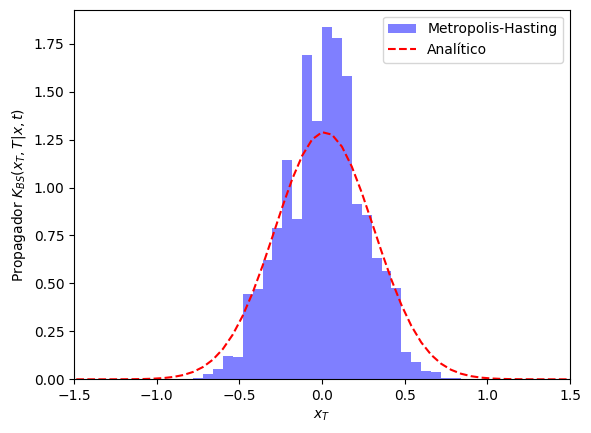
\includegraphics[width=01.0\textwidth]{MetropolisHastings.png}
\caption{Propagador de Black-Scholes en función de $x_T$. La l\'inea punteada roja corresponde al resultado obtenido anal\'iticamente mientras que el diagrama de barras corresponde a los resultados numéricos implementando Metropolis-Hastings.}
\label{fig:MetropolisHastings}
\end{figure}
En este trabajo, la implementación del algoritmo Metropolis-Hastings la realizamos en el lenguaje de programación Python. En la Fig. (\ref{fig:MetropolisHastings}) se presenta una comparación de los resultados obtenidos anal\'iticamente y num\'ericamente del propagador de Black-Scholes de en función de $x_T$ para una ventana de tiempo de un a\~no, taza libre de riesgo 0,03, volatilidad 0,3 en dimensión 5 y con un número de iteraciones igual a 1000000.

\section{Conclusiones}

En este trabajo hemos introducido el concepto de integrales de camino para la valuaci\'on de opcines financieras. Obtuvimos a partir de este enfoque el propagador de Black-Scholes de manera anal\'itica y utilizando la convoluci\'on del propagador contra la funci\'on de payoff derivamos de una manera elegante el teorema fundamental de la valuaci\'on de activos. Por otra parte, implementamos el algoritmo de Metropolis-Hasting con el lenguaje de programaci\'on Python como m\'etodo num\'erico para calcular las integrales multidimensionales que aparecen en la formulaci\'on de la integral de caminos. La comparaci\'on entre los resultados anal\'iticos y num\'ericos indican que el m\'etodo es una herramienta apropiada para la valuaci\'on de opciones m\'as complejas. Queda para el futuro la b\'usqueda de modificaciones del lagrangiano de Black-Scholes para modelar el precio de otros tipos de opciones mediante el enfoque de integrales funcionales. 

% ---------------------
% Bibliografía
% ---------------------

% Secuencia para compilar:
% 1. pdflatex main.tex
% 2. bibtex main.tex
% 3. pdflatex main.tex
% 4. pdflatex main.tex

\bibliographystyle{plain}
\bibliography{bibliography.bib}

%\end{multicols}

% ---------------------
% Fin del documento
% ---------------------

\end{document}
